\documentclass{article}
\usepackage{amsmath }
\usepackage{tikz}

\begin{document}

    \begin{center}
        \Huge
        Cardioid
        \bigskip
        \normalsize
        
        Polar equation:
        \[r\left(\theta\right)=2\left(1-\cos\theta\right)\]
        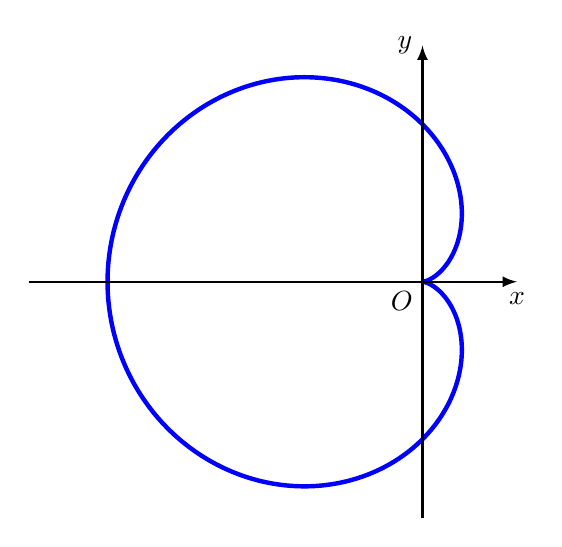
\begin{tikzpicture}[scale=1]
            \draw[color=blue, ultra thick, domain=0:360,smooth,variable=\t, samples=300] 
                plot ({\t}:{2*(1-cos(\t))});
    
            \draw[thick, ->, >=latex] (-5,0) -- (1.2,0) node[below]{\(x\)};
            \draw[thick, ->, >=latex] (0,-3) -- (0,3) node[left]{\(y\)};        
            \node at (0,0) [below left]{\(O\)};
        \end{tikzpicture}    
    \end{center}

\end{document}
